\section{Machine Learning: Window approach}

The goal of this module is to product an alternative to the grammatical approach to product triples from English sentences.

We used machine learning algorithms in order to produce triples from scratch, i.e. without any grammatical library like \Stanford.


Motivations come from three points:
\begin{itemize}
\item Because triples are linked to the semantic of the sentence, and not directly from the grammar, we could except that avoid grammatical tools can be a good idea.
\item It has been shown that a machine learning approach can produce, for a large panel of different NLP problems, very good solutions, closed to \textit{state of the art} algorithms \cite{collobert}.
\item Grammatical approaches fail on keyword sentences, like "Barack Obama birth date" because these kind of sentences does not respect the syntax of English.
\end{itemize}

This work is based mainly on the paper "Natural Language Processing (almost) from Scratch" \cite{collobert}.

Due to the restricted amount of time, we emphasis on keywords questions (keywords questions can't be analysis with grammatical tools) and we limit ourself to a restricted version of the data model:
\begin{itemize}
\item Only one level of depth: for example the sentence "What is the birth date of the president of the United States?" will be converted to the triple: \hl{(president of the United States, birth date, ?)}. 
\item We do not support \textit{types}, and connectors like \textit{first}, \textit{sort}...
\end{itemize}
We used a look-up table and a window approach neural network as explain below. The complete package\footnote{\url{https://github.com/ProjetPP/PPP-NLP-ML-standalone/}} was written in Python 3. We use the scikit-learn library, numpy and nltk as external tool.

Our algorithm can be described with three composants: the look up table, the window approach, and the classifier.

\subsubsection{Look-up table}

The look-up table is a dictionary that associates to each word $w$ a vector $V_w \in \mathbb{R}^n$, where n is the number of parameters used to encode a word (we used $n=25$).
If two English words $w_1$ and $w_2$ are synonymous, then $||w_1-w_2||_2$ is small.

The construction of the look-up table is described in \cite{collobert} and used unsupervised machine learning techniques.
We used the precomputed look-up table found here: \url{http://metaoptimize.com/projects/wordreprs/}

We also add one parameter to know if the word starts with a capitalize character or not. Finally words are embedded in vectors of dimension 26. 

\subsubsection{Window approach}

We used a window (as explain in \cite{collobert}) that focuses on one word to classify. For example, if the sentence is "What is the birth date of the president of France?", and the word to classify is "date", for a window size of 7, the window is: "is the birth \textbf{date} of the president".


We used this window because classifier algorithms usually work with a fixed number of input parameters. 

The window size is a meta parameter to choose. This window has to be large enough that we can decide in the context of the window in which category a word is. We used a window of size 9.

\subsubsection{The classifier}

If the question is "What is the birth date of the president of France?", and the focus of the window approch is on the word "date", then the goal is to classify the word \textbf{date} into one of these four categories: \textit{subject}, \textit{predicate}, \textit{object}, \textit{to forget}.

The classification of each word of the sentence into these four categories give us finally the desired triple.

The principe of the complete algorithm can be summarize in this figure: 

\begin{figure}[!ht]
  \centering
  \caption{The neural network architecture, as described in \cite{collobert}}
  \label{sandalone:tree_four}
    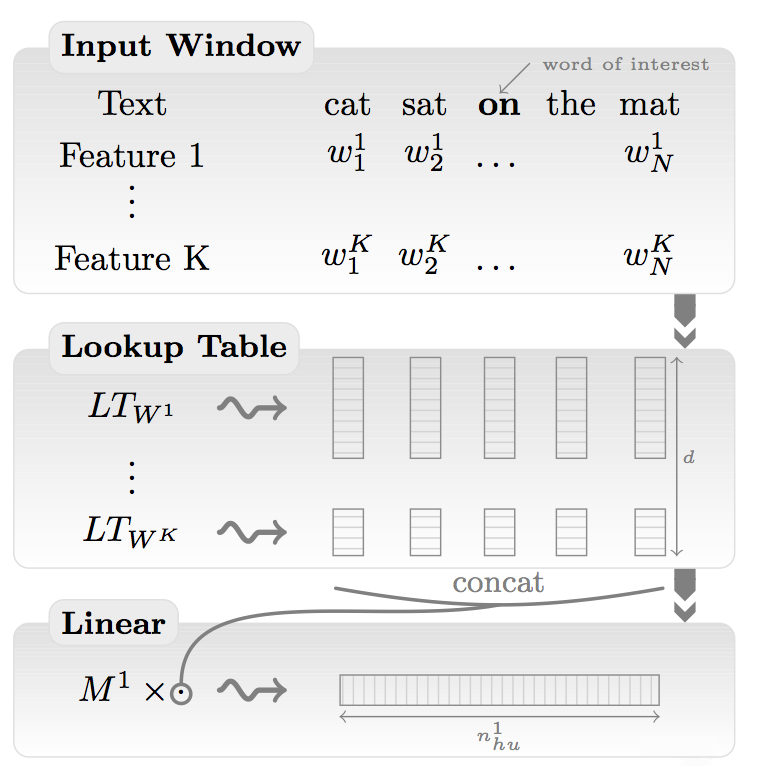
\includegraphics[scale=0.5]{../NLP-standalone-images/model.png}
\end{figure}

Because we have a a small data set of annotated questions (see below), we used a linear model, because  a linear model has the advantage to have few parameters.
For example with a window approach of size 9 and words embedded in vectors of dimension 26,  this gives us $26\times 9\times 4 = 936$ parameters to learn.

In a first time we implemented our own linear classifier, but to improve the execution time, we finally used the LDA classifier from the library scikit-learn. Few seconds of computation are needed to train successfully the model.

\subsection{Data set}

Because we used supervised algorithms, we need a data set of annotated questions.
This data set was mostly build manually, because we did not find on internet a data set that directly answering the problem of triple extraction.
Build this data set is a fastidious work. Currently our data set is composed of 300 questions.
We also wrote a script that generate keywords questions. This script give us 500 keywords questions and make the module specialized on keywords questions.


\subsection{Results}



\subsection{Future work}



